\chapter{染色质与表观遗传学}\label{ch:b3:chromatin-epigenetics}

两只来自同一窝的小鼠，遗传上完全相同，直到最后一个碱基，并排而坐：
一只苗条、棕色，另一只圆胖、
黄色，而后者日后会患糖尿病。一只三花猫身上有
橙色和黑色的斑块，尽管它皮肤的每个细胞都带有相同的两条
X 染色体。一个孩子继承了与另一个孩子相同的
第 15 号染色体缺失片段，其中一人患普拉德–威利综合征，另一人
则患安格尔曼综合征——两者的差别仅在于
缺失来自哪一位亲本。这些都不写在 DNA 序列里。它是
写\emph{在}其上：两米长的 DNA 被装进
直径十微米的细胞核中的方式，二是附着于包装蛋白
和胞嘧啶本身的小化学基团，三是把这些标记
从细胞复制给子细胞的机制。本章
所讨论的，是这第二层信息、它的分子载体，
以及它能记住什么、记不住什么的真实局限。

\section{染色质：缠绕在线轴上的 DNA}

\begin{definition}[核小体与染色质]\label{def:b3:chromatin-epigenetics:nucleosome}
\index{核小体}\index{染色质}\index{组蛋白}\index{常染色质}\index{异染色质}
\emph{染色质}是 DNA 与蛋白质构成的复合体，其中基因组存在于
真核生物细胞核中。其重复单位是
\emph{核小体}：\qty{147}{bp} 的 DNA 以左手方向缠绕
$1.65$ 圈，绕在一个\emph{组蛋白}八聚体上——即各两份小而
强碱性蛋白 H2A、H2B、H3 和 H4——其后
接 \qtyrange{20}{60}{bp} 的\emph{连接 DNA}，通向下一个核小体。第五种
组蛋白 H1 结合在连接 DNA 进入和离开核心颗粒处，并帮助
核小体彼此靠拢压缩。每个核心组蛋白都带有一段
无固定结构的氨基端\emph{尾部}，约含 \numrange{20}{40}
个残基，伸出颗粒之外。染色较浅、包装疏松并
正在转录的染色质称为\emph{常染色质}；
包装致密、复制较晚且大多沉默的染色质，
位于着丝粒、端粒和重复序列处的，称为\emph{异染色质}。
\end{definition}

\begin{proof}[证据]
休伊什和伯戈因（1973）用内源性核酸酶消化大鼠肝细胞核，
并发现 DNA 并非弥散成一片，而是呈梯状
片段，其长度为约 \qty{200}{bp} 的整数倍：
DNA 在规则间隔处受到保护，只在间隔之间被切开。
科恩伯格（1974）表明，受保护的单位是一个由八个
\omterm{def:b3:chromatin-epigenetics:nucleosome}{组蛋白}构成、约 \qty{200}{bp} 的颗粒，轻度铺展的\omterm{def:b3:chromatin-epigenetics:nucleosome}{染色质}的电镜照片
显示出“串珠”结构。卢格及其
同事（1997）解析了核心颗粒的晶体结构，分辨率为
\qty{2.8}{\angstrom}：\qty{147}{bp}，八聚体的尾部穿过
DNA 螺旋环之间伸出。
\end{proof}

\begin{omfigure}
\begin{tikzpicture}[every node/.style={font=\scriptsize}, >=stealth]
  % beads on a string
  \foreach \x/\y in {0/0, 2.2/0.5, 4.4/0, 6.6/0.5, 8.8/0} {
    \fill[omDef!30] (\x,\y) circle (0.42);
    \draw[very thick, omThm!70!black] (\x,\y) circle (0.5);
  }
  \draw[very thick, omThm!70!black] (-1.1,-0.1) -- (0-0.47,-0.17);
  \draw[very thick, omThm!70!black] (0.47,-0.17) -- (2.2-0.47,0.33);
  \draw[very thick, omThm!70!black] (2.67,0.33) -- (4.4-0.47,-0.17);
  \draw[very thick, omThm!70!black] (4.87,-0.17) -- (6.6-0.47,0.33);
  \draw[very thick, omThm!70!black] (7.07,0.33) -- (8.8-0.47,-0.17);
  \draw[very thick, omThm!70!black] (9.27,-0.17) -- (10.4,-0.1);
  % tails
  \foreach \x/\y in {0/0, 4.4/0, 8.8/0} { \draw[omProp, thick] (\x,\y+0.5) .. controls (\x-0.2,\y+0.9) .. (\x+0.1,\y+1.15); \draw[omProp, thick] (\x,\y-0.5) .. controls (\x+0.2,\y-0.9) .. (\x-0.1,\y-1.15); }
  \foreach \x/\y in {2.2/0.5, 6.6/0.5} { \draw[omProp, thick] (\x,\y+0.5) .. controls (\x-0.2,\y+0.9) .. (\x+0.1,\y+1.15); }
  % H1
  \fill[omMeth!70!black] (1.55,0.05) circle (0.12); \fill[omMeth!70!black] (5.95,0.05) circle (0.12);
  % labels
  \node[above, align=center] at (2.2,1.75) {组蛋白尾部 \\（乙酰化、甲基化）};
  \node[below, align=center] at (4.4,-1.35) {核心颗粒：八聚体 \\$+$ \qty{147}{bp}，$1.65$ 圈};
  \node[below, align=center] at (7.7,-0.55) {连接 DNA\\\qtyrange{20}{60}{bp}};
  \node[below] at (5.95,-0.1) {H1};
  \draw[<->] (-0.5,-2.2) -- (2.2-0.5,-2.2) node[midway, below] {重复单位 $\approx \qty{200}{bp}$，\qty{11}{nm}};
  \draw[gray] (-0.5,-1.95) -- (-0.5,-2.35); \draw[gray] (1.7,-1.95) -- (1.7,-2.35);
\end{tikzpicture}

{\small \qty{10}{nm} 纤维：\omterm{def:b3:chromatin-epigenetics:nucleosome}{核小体}核心（蓝色）位于连续的
DNA（红色）之上，每个珠子都是\omterm{def:b3:chromatin-epigenetics:nucleosome}{组蛋白}八聚体，其尾部（橙色）
向外伸出，连接\omterm{def:b3:chromatin-epigenetics:nucleosome}{组蛋白} H1（绿色）位于进出点。约六个
\omterm{def:b3:chromatin-epigenetics:nucleosome}{核小体}所占长度，相当于 \qty{1200}{bp} 裸 DNA 的长度。}
\end{omfigure}

\begin{omfigure}
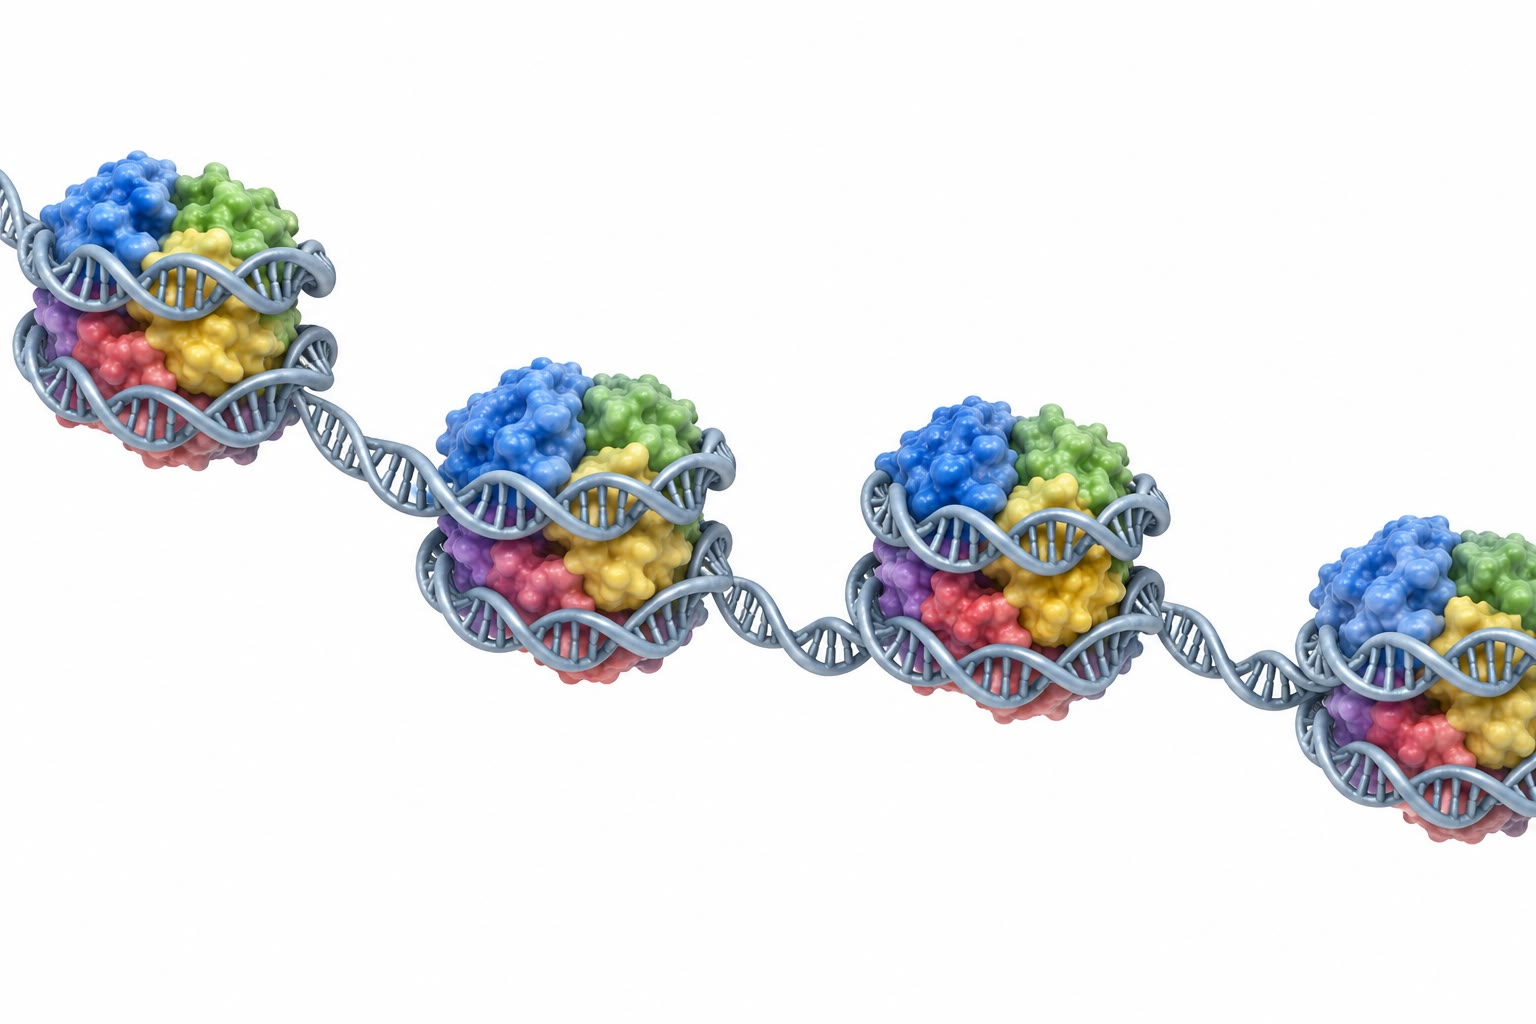
\includegraphics[width=0.6\linewidth]{images/book5/ai/b5-01-nucleosomes.jpg}

{\small 分子尺度上的\omterm{def:b3:chromatin-epigenetics:nucleosome}{染色质}：双螺旋缠绕在
相继\omterm{def:b3:chromatin-epigenetics:nucleosome}{组蛋白}核心之上，即核酸酶梯状实验所揭示的
“串珠”结构。}
\end{omfigure}

\begin{proposition}[压缩层次]\label{prop:b3:chromatin-epigenetics:compaction}
\index{包装比}\index{染色质环}\index{拓扑关联结构域}
\omterm{def:b3:chromatin-epigenetics:nucleosome}{染色质}结构的\emph{\omterm{prop:b3:chromatin-epigenetics:compaction}{包装比}}是其所含
DNA 的长度与该结构长度之比。绕成
\qty{10}{nm} 纤维时比值约为 $6$：一个
\qty{200}{bp} 重复单位的 \qty{68}{nm} 被压缩为一个 \qty{11}{nm} 的珠子。在
间期细胞核中，纤维并非卷绕成规则的较粗纤维，
正如教科书长期所绘，而是折叠成\emph{\omterm{prop:b3:chromatin-epigenetics:compaction}{染色质环}}，
长为数十至数百千碱基，其基部由环形黏连蛋白复合体
和 DNA 结合蛋白 CTCF 固定；这些环聚集
成\emph{\omterm{prop:b3:chromatin-epigenetics:compaction}{拓扑关联结构域}}（TAD），约一兆碱基，
其中基因与调控元件相遇的频率远高于与区域外
任何元件相遇。有丝分裂染色体是最致密的状态，其
\omterm{prop:b3:chromatin-epigenetics:compaction}{包装比}接近 \num{10000}：一条普通人类染色体中的 \qty{4}{cm} DNA
被折叠成一根 \qty{4}{\micro m}
长的棒状结构。
\end{proposition}

\begin{example}[十微米内的两米]\label{ex:b3:chromatin-epigenetics:two-metres}
人类二倍体细胞核含有 $6.4\times 10^{9}$ 个碱基对。
每个碱基对 \qty{0.34}{nm}，共 \qty{2.2}{m} 双螺旋，
置于直径约 \qty{10}{\micro m} 的细胞核中。它被装进
$6.4\times 10^{9}/200 \approx 3.2\times 10^{7}$ 个\omterm{def:b3:chromatin-epigenetics:nucleosome}{核小体}，每个
携带约 \qty{108}{kDa} \omterm{def:b3:chromatin-epigenetics:nucleosome}{组蛋白}，对应 \qty{96}{kDa} 的 DNA
（\qty{147}{bp}，按每对 \qty{650}{Da} 计）：细胞核中的\omterm{def:b3:chromatin-epigenetics:nucleosome}{组蛋白}
质量与 DNA 大致相当。把 DNA 本身看作直径
\qty{2}{nm} 的圆柱体，其体积仅约 \qty{7}{\micro m^3}，
约占半径 \qty{5}{\micro m} 的球形细胞核的 \qty{1}{\%}；
包装的难题在于缠绕与可及，而非空间。
\end{example}

\section{组蛋白密码}

\begin{definition}[组蛋白修饰]\label{def:b3:chromatin-epigenetics:histone-code}
\index{组蛋白密码}\index{乙酰化}\index{组蛋白甲基化}\index{书写器}\index{阅读器}\index{擦除器}
\omterm{def:b3:chromatin-epigenetics:nucleosome}{组蛋白}尾部的残基会发生共价修饰：
赖氨酸的\emph{乙酰化}（中和其正电荷，
并松开对 DNA 的束缚），赖氨酸和精氨酸的\emph{甲基化}
（可加一个、两个或三个甲基，电荷不变），
丝氨酸的磷酸化，赖氨酸的泛素化。一种修饰
按\omterm{def:b3:chromatin-epigenetics:nucleosome}{组蛋白}、残基和基团命名：H3K4me3 表示\omterm{def:b3:chromatin-epigenetics:nucleosome}{组蛋白} H3 的第 4 位赖氨酸
被三甲基化；H3K27ac 表示 H3 的第 27 位赖氨酸被乙酰化。\emph{\omterm{def:b3:chromatin-epigenetics:nucleosome}{组蛋白}
密码}指修饰组合与其所在基因状态之间的相关性：
活跃启动子和增强子处有 H3K4me3 与 H3K27ac，
转录基因的基因体上有 H3K36me3，组成型\omterm{def:b3:chromatin-epigenetics:nucleosome}{异染色质}上有 H3K9me3，
发育中被沉默的基因上有 H3K27me3。
添加修饰的酶称为\emph{书写器}（\omterm{def:b3:chromatin-epigenetics:nucleosome}{组蛋白}乙酰转移酶，
HAT；甲基转移酶），移除修饰的酶
称为\emph{擦除器}（\omterm{def:b3:chromatin-epigenetics:nucleosome}{组蛋白}去乙酰化酶，HDAC；去甲基化酶），而
结合修饰并作用于它的蛋白称为\emph{阅读器}：
\emph{溴结构域}结合乙酰化赖氨酸，\emph{\omterm{def:b3:chromatin-epigenetics:nucleosome}{染色质}结构域}
结合甲基化赖氨酸。
\end{definition}

\begin{proposition}[标记是被阅读的，而不只是被感知]\label{prop:b3:chromatin-epigenetics:readers}
\index{HP1}\index{多梳}\index{PRC2}\index{Trithorax}
\omterm{def:b3:chromatin-epigenetics:histone-code}{乙酰化}部分通过静电作用发挥作用——\omterm{def:b3:chromatin-epigenetics:histone-code}{乙酰化}的尾部对 DNA 的束缚较弱，
纤维随之打开——但大多数标记通过
招募\omterm{def:b3:chromatin-epigenetics:histone-code}{阅读器}起作用。H3K9me3 被
\emph{\omterm{def:b3:chromatin-epigenetics:nucleosome}{异染色质}蛋白 \omterm{prop:b3:chromatin-epigenetics:readers}{HP1}} 的\omterm{def:b3:chromatin-epigenetics:nucleosome}{染色质}结构域结合，该蛋白二聚化并
连接相邻的\omterm{def:b3:chromatin-epigenetics:nucleosome}{核小体}，并招募恰好在下一个\omterm{def:b3:chromatin-epigenetics:nucleosome}{核小体}上写入 H3K9me3 的
甲基转移酶（SUV39H）：标记沿纤维扩散，
直到遇到边界，并压缩其所覆盖的区域。
H3K27me3 由\emph{\omterm{prop:b3:chromatin-epigenetics:readers}{多梳}抑制复合体 2}
（\omterm{prop:b3:chromatin-epigenetics:readers}{PRC2}，催化亚基为 EZH2）书写，由 PRC1 识别，PRC1 使 H2A 泛素化，
并压缩纤维，而该复合体本身受其所产生标记的
刺激；\emph{\omterm{prop:b3:chromatin-epigenetics:readers}{Trithorax}} 类蛋白家族书写与之相反的
H3K4me3，并使特定细胞类型的发育基因保持
开启。每一个这样的环路——\omterm{def:b3:chromatin-epigenetics:histone-code}{阅读器}招募\omterm{def:b3:chromatin-epigenetics:histone-code}{书写器}——都是一种
正反馈，使一旦建立的状态能够自我维持，这正是
可遗传标记所需要的。
\end{proposition}

\begin{omfigure}
\begin{tikzpicture}[every node/.style={font=\scriptsize}, >=stealth]
  % nucleosomes with tails
  \foreach \x in {0,2,4,6} { \draw[thick, omDef, fill=omDef!20] (\x,0) circle (0.45); \draw[omProp, thick] (\x,0.45) -- (\x,1.15); }
  % marks
  \fill[omThm] (2,1.15) circle (0.11); \fill[omThm] (4,1.15) circle (0.11);
  \fill[omMeth!80!black] (0,1.15) circle (0.11);
  \node[left] at (-0.5,1.15) {ac};
  \node[right, align=left] at (6.15,1.15) {me3};
  % HP1 reader
  \draw[thick, fill=omExo!30] (2.6,1.7) ellipse (0.5 and 0.25); \node at (2.6,1.7) {阅读器};
  \draw[thick, fill=omExo!30] (4.2,2.35) ellipse (0.55 and 0.25); \node at (4.2,2.35) {书写器};
  \draw[->, thick] (2.9,1.9) -- (3.75,2.2);
  \draw[->, thick, omThm] (4.6,2.15) .. controls (5.6,2.0) and (6.1,1.8) .. (6.05,1.3);
  \node[right, align=left, font=\scriptsize] at (6.6,2.0) {扩散至 \\下一个核小体};
  \draw[->, thick, gray] (2.2,1.3) -- (2.45,1.5);
  % eraser
  \draw[thick, fill=omExo!30] (0.6,2.2) ellipse (0.5 and 0.25); \node at (0.6,2.2) {擦除器};
  \draw[->, thick, omMeth!80!black] (0.3,2.0) -- (0.05,1.35);
  % DNA
  \draw[very thick, omThm!70!black] (-0.9,-0.3) -- (-0.45,-0.05) (0.45,-0.05) -- (1.55,-0.05) (2.45,-0.05) -- (3.55,-0.05) (4.45,-0.05) -- (5.55,-0.05) (6.45,-0.05) -- (7.2,-0.3);
  \node[below, align=center] at (0,-0.6) {开放：乙酰基 \\中和一个电荷};
  \node[below, align=center] at (5,-0.6) {闭合：H3K9me3 被 HP1 识别，\\进而招募 K9 甲基转移酶};
\end{tikzpicture}

{\small \omterm{def:b3:chromatin-epigenetics:histone-code}{书写器}–\omterm{def:b3:chromatin-epigenetics:histone-code}{阅读器}–\omterm{def:b3:chromatin-epigenetics:histone-code}{擦除器}的逻辑。结合在某个\omterm{def:b3:chromatin-epigenetics:nucleosome}{核小体}标记上的\omterm{def:b3:chromatin-epigenetics:histone-code}{阅读器}招募\omterm{def:b3:chromatin-epigenetics:histone-code}{书写器}，
\omterm{def:b3:chromatin-epigenetics:histone-code}{书写器}在下一个\omterm{def:b3:chromatin-epigenetics:nucleosome}{核小体}上写入相同标记，因此状态得以扩散并自我复制；\omterm{def:b3:chromatin-epigenetics:histone-code}{擦除器}则与之对抗。
乙酰基（绿色）使纤维打开；
H3K9me3（红色）使纤维闭合。}
\end{omfigure}

\begin{method}[染色质免疫沉淀（ChIP）]\label{met:b3:chromatin-epigenetics:chip}
\index{ChIP}\index{染色质免疫沉淀}
为绘制标记或蛋白质在基因组上的位置，依次进行：(1) 在活细胞中
用甲醛使蛋白质与 DNA 交联；(2) 将\omterm{def:b3:chromatin-epigenetics:nucleosome}{染色质}剪切成
几百个碱基对的片段；(3) 用针对某一标记（如
H3K27me3）的抗体沉淀这些片段，抗体结合在
磁珠上；(4) 逆转交联并纯化 DNA；(5) 对其测序
（ChIP-seq），沿基因组计数读段：峰即为标记所在之处。
以不加抗体的输入 DNA 为对照，用于设定
背景。分辨率由片段大小决定，约为一个
\omterm{def:b3:chromatin-epigenetics:nucleosome}{核小体}。
\end{method}

\begin{remark}[“密码”还是相关性]\label{rem:b3:chromatin-epigenetics:code}
“密码”一词言过其实。许多标记是转录的结果，
而非转录的原因（H3K36me3 由
随聚合酶移动的甲基转移酶沉积），移除\omterm{def:b3:chromatin-epigenetics:histone-code}{书写器}
通常对表达的影响远小于标记分布所暗示的程度，
已确证的是，少数标记——H3K9me3、
H3K27me3 和下文的 DNA 甲基化——携带自我传播的
沉默信号，其持续时间超过了建立它的信号。
\end{remark}

\section{DNA 甲基化与标记的复制}

\begin{definition}[DNA 甲基化]\label{def:b3:chromatin-epigenetics:methylation}
\index{DNA 甲基化}\index{CpG}\index{CpG 岛}\index{DNMT1}\index{维持甲基化}\index{从头甲基化}
在脊椎动物中，甲基几乎只加到胞嘧啶的第 5 位碳原子上，
且仅限于二核苷酸\emph{CpG}（同一条链上的 C 后接 G），
该序列与其互补序列相同，因此被甲基化的
CpG 通常在两条链上都被甲基化。人类细胞中约有 \qtyrange{70}{80}{\%}
的 CpG 被甲基化，被甲基化的启动子
处于沉默状态：甲基由甲基-CpG 结合蛋白识别
（MeCP2、MBD1--4），这些蛋白招募 HDAC 和 H3K9 甲基转移酶，它们
还直接阻断多种转录因子。例外是
\emph{CpG 岛}，长约一千碱基的片段，富含 G 和 C，
且富含 CpG，位于大多数管家基因的启动子处，
在正常细胞中保持未甲基化。甲基由
\emph{DNA 甲基转移酶}写入：DNMT3A 和 DNMT3B 对未甲基化位点进行\emph{从头
甲基化}，\emph{DNMT1} 则偏好
半甲基化的 CpG——一条链甲基化、另一条未甲基化 ---，
由\emph{维持甲基化}在复制叉之后完成。去除甲基化的方式
有两种：被动去除，即复制时不进行维持；或主动去除，由 TET
酶完成，它们将 5-甲基胞嘧啶氧化为 5-羟甲基胞嘧啶，并继续
氧化，直至碱基切除修复将其替换为普通胞嘧啶。
\end{definition}

\begin{example}[基因组为何缺少 CpG]\label{ex:b3:chromatin-epigenetics:cpg-deficit}
人类基因组的 G$+$C 含量为 \qty{42}{\%}，因此若碱基彼此独立，
\omterm{def:b3:chromatin-epigenetics:methylation}{CpG} 出现的频率应为 $0.21\times 0.21 \approx 0.044$，
即在二倍体基因组中约出现 $2.8\times 10^{8}$ 次。实际观察到的数目
约为 $5.6\times 10^{7}$，仅为其五分之一。原因在于标记
本身：甲基化胞嘧啶失去氨基后，
变为胸腺嘧啶，这是一种修复系统无法识别为错误的正常碱基；而
未甲基化的胞嘧啶脱氨基生成尿嘧啶，随即被切除。经过
漫长的演化，甲基化的 \omterm{def:b3:chromatin-epigenetics:methylation}{CpG} 已突变为 TpG 和 CpA，
只有未甲基化的 \omterm{def:b3:chromatin-epigenetics:methylation}{CpG} 岛保留了原有的 \omterm{def:b3:chromatin-epigenetics:methylation}{CpG}。这一标记
在序列中留下了自己的印记。
\end{example}

\begin{theorem}[甲基化状态在分裂中的维持]\label{thm:b3:chromatin-epigenetics:maintenance}
\index{表观遗传记忆}\index{马尔可夫链!甲基化}
考虑一个 \omterm{def:b3:chromatin-epigenetics:methylation}{CpG} 位点，沿一条细胞谱系追踪。
每次分裂时，若模板链上的胞嘧啶已甲基化，则新链上的胞嘧啶
以概率 $\mu$ 被甲基化（维持效率）；若模板链未甲基化，则
以概率 $\delta$ 被甲基化（\omterm{def:b3:chromatin-epigenetics:methylation}{从头甲基化}速率）。
设 $p_{n}$ 为该位点在 $n$
次分裂后被甲基化的概率。则
\[
p_{n+1} = \mu\, p_{n} + \delta\,(1 - p_{n}),
\qquad
p_{n} = p^{*} + (p_{0} - p^{*})\,(\mu - \delta)^{n},
\qquad
p^{*} = \frac{\delta}{1 - \mu + \delta}.
\]
每个位点都会趋向于同一平衡值 $p^{*}$，无论其起始状态如何，
而初始状态的记忆
以公比 $\mu - \delta$ 按几何级数衰减。一个标记
大约能被记住 $1/(1 - \mu + \delta)$ 次分裂；忠实记住
位点之间的\emph{差异}，因此需要 $\mu$ 非常接近
$1$，$\delta$ 非常接近 $0$，或者存在一种反馈，使 $\mu$ 与
$\delta$ 依赖于邻近区域的状态。
\end{theorem}
\begin{proof}
该递推式是对模板两种状态应用全概率公式的结果。
其不动点满足 $p^{*} = \mu p^{*} + \delta(1 -
p^{*})$，由此得 $p^{*}(1 - \mu + \delta) = \delta$。将递推式减去不动点方程，
得 $p_{n+1} - p^{*} = (\mu -
\delta)(p_{n} - p^{*})$，迭代即得闭式解。由于
$0 \le \delta \le \mu \le 1$，比值 $\mu - \delta$ 位于 $[0,1]$ 内，
偏差随之缩小；每隔 $\ln 2 / (-\ln(\mu -
\delta)) \approx \ln 2/(1 - \mu + \delta)$ 次分裂偏差减半，当 $\mu -
\delta$ 接近 $1$ 时。
\end{proof}

\begin{example}[数值]\label{ex:b3:chromatin-epigenetics:maintenance-numbers}
哺乳动物细胞的实测值为：在典型 \omterm{def:b3:chromatin-epigenetics:methylation}{CpG} 位点处，$\mu \approx 0.99$ 和
$\delta \approx 0.02$（每次分裂）。于是 $p^{*} =
0.02/0.03 \approx 0.67$，接近全基因组的甲基化比例，
且 $\mu - \delta = 0.97$：一个完全甲基化的位点若仅交由机制维持，
则经过 $\ln 2 /
0.03 \approx 23$ 次分裂后便回到平均水平的一半。一个沉默的启动子
若要在细胞一生的数百次分裂中保持沉默，仅靠 \omterm{def:b3:chromatin-epigenetics:methylation}{DNMT1} 是不够的：
甲基化 \omterm{def:b3:chromatin-epigenetics:methylation}{CpG} 的\omterm{def:b3:chromatin-epigenetics:histone-code}{阅读器}会招募 H3K9 甲基化，而 H3K9
的\omterm{def:b3:chromatin-epigenetics:histone-code}{阅读器}会招募 DNMT3，于是一个由标记密集形成的岛会将自身的
$\mu$ 提高至接近 $1$，并将邻近的 $\delta$ 降低至接近 $0$。
相反，若细胞失去 \omterm{def:b3:chromatin-epigenetics:methylation}{DNMT1}，标记便被动丢失：
当 $\mu = \delta = 0$ 时，甲基化链的比例
每次分裂减半。
\end{example}

\begin{omfigure}
\begin{tikzpicture}[every node/.style={font=\scriptsize}, >=stealth]
  % left: replication scheme
  \begin{scope}
    \draw[very thick, omThm!70!black] (0,1.2) -- (2.4,1.2); \draw[very thick, omThm!70!black] (0,0.9) -- (2.4,0.9);
    \foreach \x in {0.5,1.2,1.9} { \fill[omDef] (\x,1.2) circle (0.09); \fill[omDef] (\x,0.9) circle (0.09); }
    \node[above] at (1.2,1.3) {亲代：两条链均甲基化};
    \draw[->, thick] (1.2,0.75) -- (1.2,0.15) node[midway, right] {复制};
    \draw[very thick, omThm!70!black] (0,-0.1) -- (2.4,-0.1); \draw[very thick, gray] (0,-0.4) -- (2.4,-0.4);
    \foreach \x in {0.5,1.2,1.9} { \fill[omDef] (\x,-0.1) circle (0.09); \draw[omDef] (\x,-0.4) circle (0.09); }
    \node[left] at (-0.1,-0.25) {半甲基化};
    \draw[->, thick] (1.2,-0.85) -- (1.2,-1.45) node[midway, right, align=left] {DNMT1，概率 $\mu$\\每位点};
    \draw[very thick, omThm!70!black] (0,-1.7) -- (2.4,-1.7); \draw[very thick, gray] (0,-2.0) -- (2.4,-2.0);
    \foreach \x in {0.5,1.9} { \fill[omDef] (\x,-1.7) circle (0.09); \fill[omDef] (\x,-2.0) circle (0.09); }
    \fill[omDef] (1.2,-1.7) circle (0.09); \draw[omDef] (1.2,-2.0) circle (0.09);
    \node[below, align=center] at (1.2,-2.1) {恢复，漏掉一个位点：\\子代的新链};
  \end{scope}
  % right: decay plot
  \begin{scope}[xshift=5.0cm, yshift=-2.3cm]
  \begin{axis}[
    width=6.6cm, height=4.6cm, axis lines=left,
    xmin=0, xmax=100, ymin=0, ymax=1.05,
    xlabel={分裂次数 $n$},
    xlabel style={font=\scriptsize, at={(axis description cs:0.5,-0.1)}, anchor=north},
    tick label style={font=\scriptsize}, xtick={0,25,50,75,100}, ytick={0,0.5,0.67,1},
    yticklabels={0,0.5,$p^{*}$,1}, clip=false,
  ]
  \addplot[very thick, omDef, domain=0:100, samples=60] {0.6667 + 0.3333*0.97^x};
  \addplot[very thick, omThm, domain=0:100, samples=60] {0.6667 - 0.6667*0.97^x};
  \addplot[dashed, gray, domain=0:100, samples=2] {0.6667};
  \addplot[thick, omMeth!80!black, domain=0:100, samples=60] {0.6667 + 0.3333*0.998^x};
  \node[font=\scriptsize] at (axis cs:-9,1.1) {$p_{n}$};
  \node[font=\scriptsize, omDef, anchor=south west] at (axis cs:45,0.82) {已甲基化起始，$\mu = 0.99$};
  \node[font=\scriptsize, omThm, anchor=north west] at (axis cs:50,0.30) {未甲基化起始};
  \node[font=\scriptsize, omMeth!80!black, anchor=south west] at (axis cs:30,1.02) {有反馈，$\mu = 0.999$};
  \end{axis}
  \end{scope}
\end{tikzpicture}

{\small 左：\omterm{def:b3:chromatin-epigenetics:methylation}{维持甲基化}。复制之后，每个 \omterm{def:b3:chromatin-epigenetics:methylation}{CpG} 都呈
半甲基化状态；\omterm{def:b3:chromatin-epigenetics:methylation}{DNMT1} 以
每位点概率 $\mu$ 将标记复制到新链上。右图：一个位点随分裂次数的
变化情况，对于 $\mu = 0.99$、$\delta = 0.02$（蓝色为起始已甲基化，红色为
起始未甲基化）——两者都收敛于 $p^{*} = 0.67$——以及一个
邻近区域反馈将 $\mu$ 提高至 $0.999$ 的位点（绿色）。}
\end{omfigure}

\begin{method}[读取甲基化：亚硫酸氢盐测序]\label{met:b3:chromatin-epigenetics:bisulfite}
\index{亚硫酸氢盐测序}
单靠测序无法看到甲基。用亚硫酸氢钠处理变性的 DNA，
未甲基化的胞嘧啶脱氨基成为尿嘧啶，
经 PCR 后被读为 T，而 5-甲基胞嘧啶受到保护，
仍被读为 C。对转化后的 DNA 进行测序，并与参考序列比较：
凡仍为 C 的位点即被甲基化，凡变为 T 的则未被甲基化。
若在全基因组范围内进行（全基因组\omterm{met:b3:chromatin-epigenetics:bisulfite}{亚硫酸氢盐测序}），
则可在单碱基分辨率下得到单倍体基因组中每个 \omterm{def:b3:chromatin-epigenetics:methylation}{CpG}（共 $2.8\times 10^{7}$ 个）的
甲基化状态，以样本中细胞的
比例表示。
\end{method}

\section{X 染色体失活与基因组印记}

\begin{definition}[X 染色体失活]\label{def:b3:chromatin-epigenetics:x-inactivation}
\index{X 染色体失活}\index{巴氏小体}\index{Xist}\index{剂量补偿}
在雌性哺乳动物中，每个体细胞的两条 X 染色体之一
在发育早期即被转录沉默，这是一种
\emph{剂量补偿}，使 X 连锁基因的表达在 XX 雌性与 XY 雄性之间
趋于一致。被沉默的染色体压缩成一个致密体，
紧贴核膜，即\emph{巴氏小体}。
哪条 X 染色体被沉默是随机的（在胚胎本体中），
一旦选定，即通过克隆方式遗传给该细胞的所有后代。
失活由 \emph{Xist} 启动，它是一种 \qty{17}{kb} 的非编码 RNA，
由将被沉默的染色体上的 X 失活中心转录而来，
它以顺式方式包被该染色体，招募 Polycomb（H3K27me3）、
\omterm{def:b3:chromatin-epigenetics:nucleosome}{组蛋白}变体 macroH2A，最终是启动子的 DNA 甲基化，
此后沉默状态得以维持，无需 Xist 在每次分裂时
再次参与。人类 X 连锁基因中约 \qty{15}{\%} 的
基因部分或全部逃逸失活。
\end{definition}

\begin{proof}[证据]
巴尔与伯特伦（1949）在雌性
而非雄性猫的神经元细胞核中注意到一个致密体。大野乾（1959）证明其为一条完整的 X
染色体凝缩而成。莱昂（1961）将这些证据串联起来：雌性
在 X 连锁毛色基因上为杂合子的小鼠，毛色呈镶嵌状，
斑块分别表达其中一个等位基因，因此每个斑块都是一个克隆，
其中始终是同一条 X 染色体被沉默；同样的情况也见于玳瑁猫或三花猫的
橙黑斑块，其橙色基因位于 X 染色体上，同样适用于携带
某一 X 连锁基因突变等位基因的女性的镶嵌状汗腺。
雄性三花猫几乎总是
XXY。
\end{proof}

\begin{omfigure}
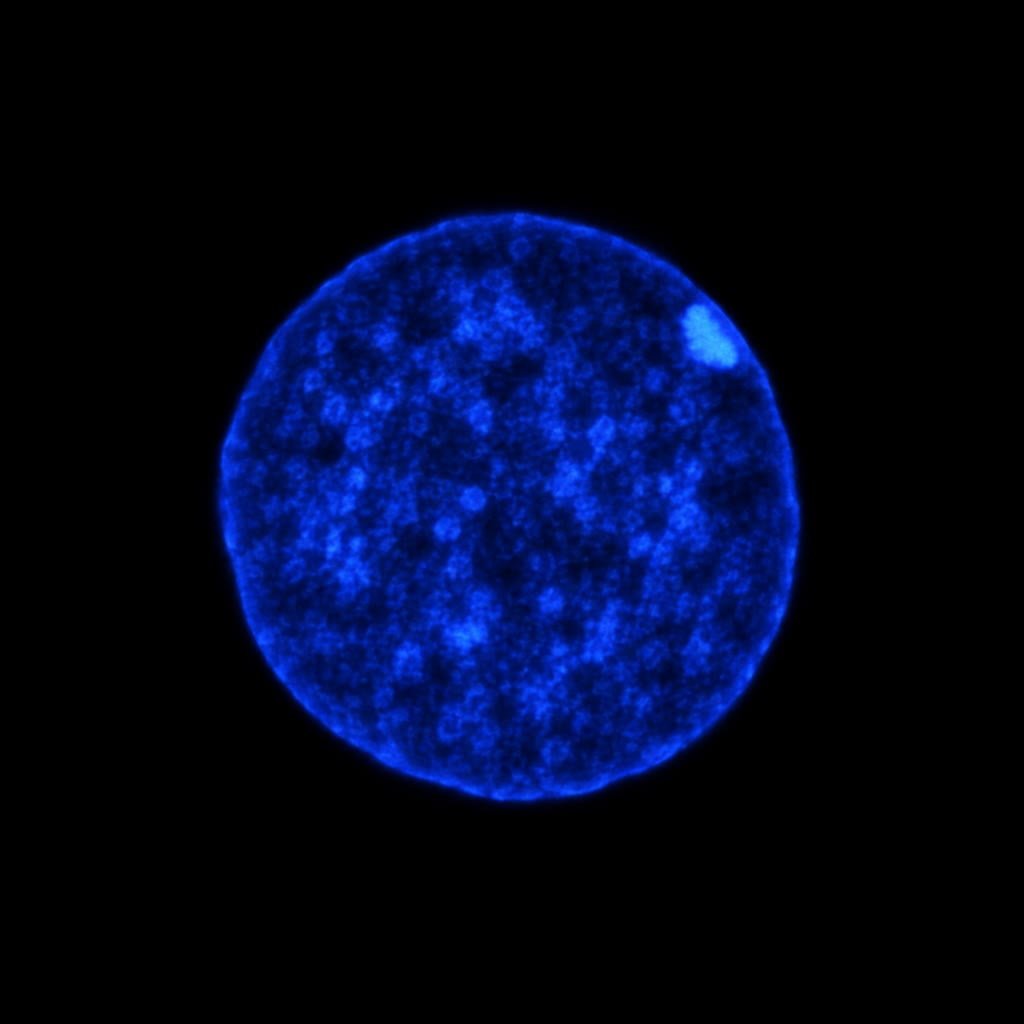
\includegraphics[width=0.42\linewidth]{images/book5/ai/b5-01-barr-body.jpg}\hspace{0.04\linewidth}
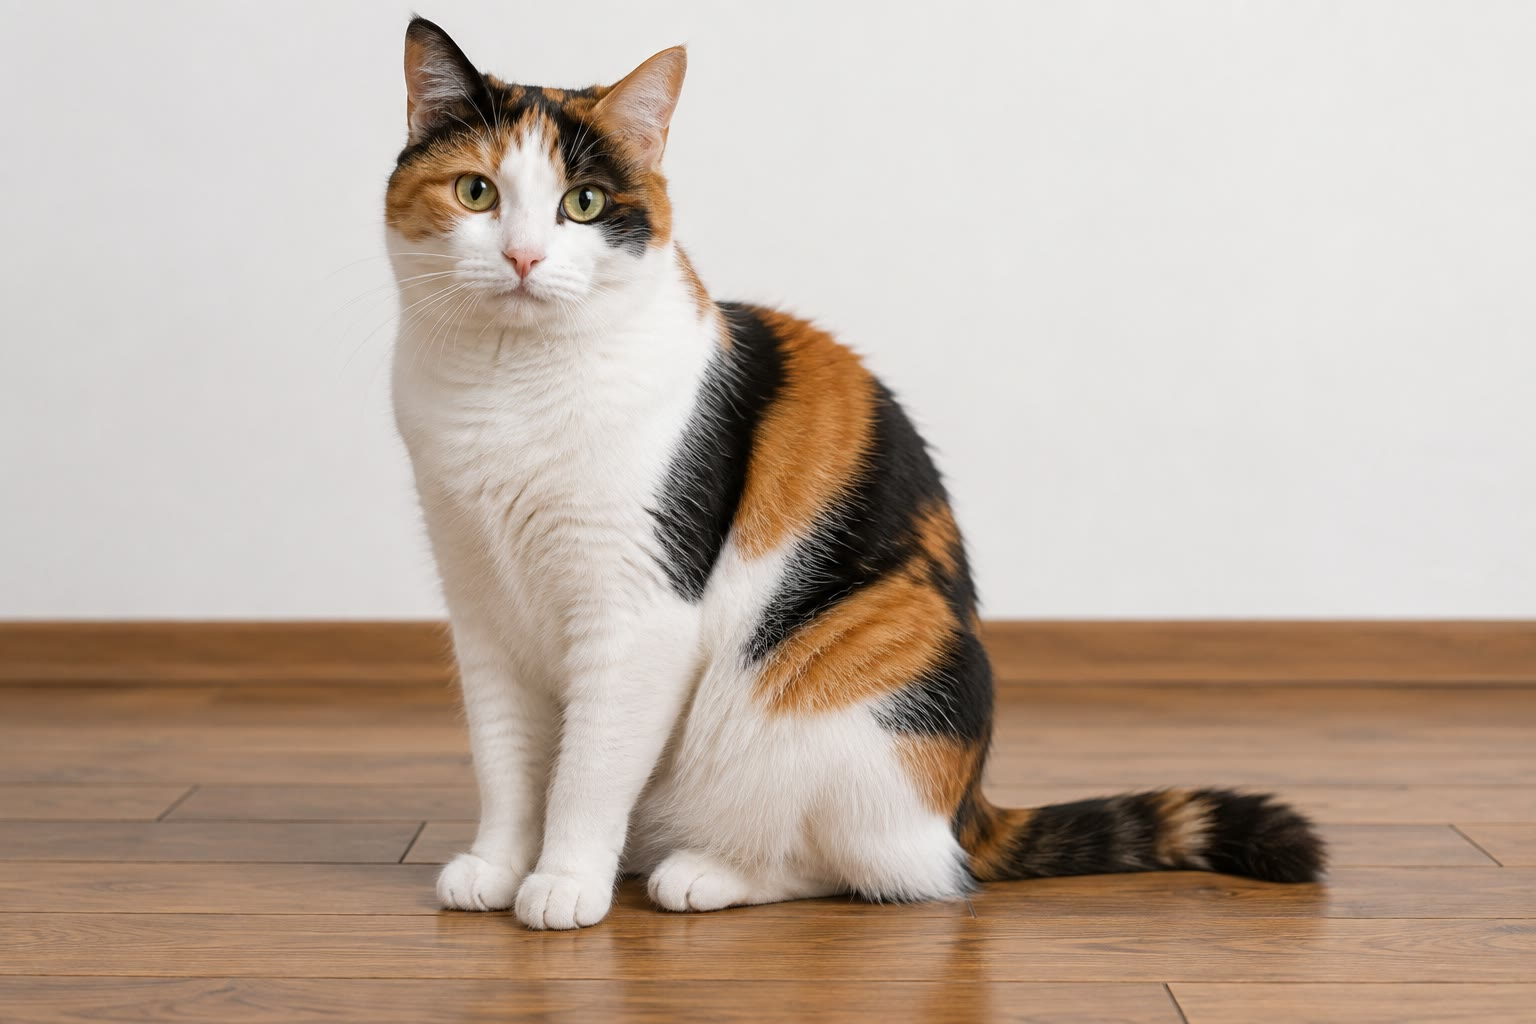
\includegraphics[width=0.5\linewidth]{images/book5/ai/b5-01-calico-cat.jpg}

{\small 左：经 DNA 染色的雌性细胞核，致密的
失活 X 染色体——即\omterm{def:b3:chromatin-epigenetics:x-inactivation}{巴氏小体}——紧贴核膜边缘。
右：三花猫。每一块橙色或黑色斑块都是一个皮肤细胞
克隆，这些细胞沉默的是同一条 X 染色体；白色则由另一个
常染色体上的斑点基因决定。}
\end{omfigure}

\begin{definition}[基因组印记]\label{def:b3:chromatin-epigenetics:imprinting}
\index{基因组印记}\index{印记控制区}\index{单亲二体}
某基因的两个等位基因中仅一个被表达时，该基因即为\emph{印记的}，
表达哪一个取决于其来源的亲本：有些
基因仅从父本拷贝表达，另一些仅从母本
拷贝表达。哺乳动物约有 \numrange{100}{200} 个印记基因，
成簇分布，每一簇由一个\emph{印记控制
区}（ICR）调控，它在一个亲本的等位基因上甲基化，
而在另一亲本上则不然。甲基化在生殖系中建立，精子中为一种模式，
卵子中为另一种模式，这些模式在下一代的生殖细胞中被擦除，
再依据该个体的性别重新建立。一个
子代若从同一亲本获得某条染色体的两个拷贝
（\emph{单亲二体}），因此其上的印记基因剂量错误，
尽管其序列完全正常。
\end{definition}

\begin{proof}[证据]
麦格拉思与索尔特，以及苏拉尼、巴顿与诺里斯（1984）各自独立地，
制得携带两个母本原核或两个父本原核的小鼠合子，
方法是在受精卵之间转移原核。两者均未发育至足月，
尽管各自都具有两套完整染色体：
雌核发育胚胎形成了尚可的胚胎，胎盘却较差，
雄核发育胚胎则是胎盘巨大而几乎没有胚胎。
双亲基因组并不等价，二者缺一不可。
卡塔纳奇与柯克（1985）利用染色体特异的\omterm{def:b3:chromatin-epigenetics:imprinting}{单亲二体}证明，
这种不等价性仅局限于某些染色体的特定区域，
这些区域正是日后找到印记基因簇的
位置。
\end{proof}

\begin{example}[\emph{Igf2}--\emph{H19} 基因簇]\label{ex:b3:chromatin-epigenetics:igf2}
\emph{Igf2}，一种胎儿生长因子，由父本
等位基因表达；其邻近基因 \emph{H19}（一种非编码 RNA）则由母本
表达。两者之间是 ICR，越过 \emph{H19} 之外则是一组共用的
增强子。在母本染色体上，ICR 未甲基化，并结合 CTCF，
它起绝缘子的作用：增强子能够作用于 \emph{H19}，
而不能作用于 \emph{Igf2}。在父本染色体上，ICR 发生甲基化（在精子中建立），
CTCF 无法结合，增强子则延伸至 \emph{Igf2}；甲基化还扩散，
使 \emph{H19} 的启动子沉默。
一个在同一生殖系中建立的标记，决定了两个基因的表达。
\end{example}

\begin{omfigure}
\begin{tikzpicture}[every node/.style={font=\scriptsize}, >=stealth]
  \foreach \yy/\lab/\ctcf in {1.6/母源染色体/1, -0.6/父源染色体/0} {
    \draw[very thick, gray] (0,\yy) -- (9.4,\yy);
    \node[left, align=right] at (-0.15,\yy) {\lab};
    \draw[thick, fill=omDef!25] (1.0,\yy-0.2) rectangle (2.6,\yy+0.2); \node at (1.8,\yy) {\emph{Igf2}};
    \draw[thick, fill=omProp!30] (4.2,\yy-0.2) rectangle (5.2,\yy+0.2); \node at (4.7,\yy) {ICR};
    \draw[thick, fill=omDef!25] (6.2,\yy-0.2) rectangle (7.4,\yy+0.2); \node at (6.8,\yy) {\emph{H19}};
    \foreach \x in {8.4,8.8,9.2} \fill[omMeth!70!black] (\x,\yy) circle (0.12);
    \node[right] at (9.55,\yy) {增强子};
  }
  % maternal: CTCF bound, enhancer -> H19
  \draw[thick, fill=omExo!35] (4.7,2.15) ellipse (0.45 and 0.22); \node at (4.7,2.15) {CTCF};
  \draw[->, thick, omMeth!70!black] (8.4,1.85) .. controls (7.8,2.5) and (7.2,2.5) .. (6.8,1.85);
  \node[above] at (7.6,2.35) {开启};
  \draw[thick, omThm] (5.3,2.3) -- (5.3,0.9); \node[omThm, below] at (5.3,0.9) {绝缘子};
  \node[omThm, above=1.0cm, align=center, font=\scriptsize] at (1.8,1.8) {\emph{胎儿生长因子}沉默};
  % paternal: ICR methylated
  \foreach \x in {4.35,4.6,4.85,5.1} \fill[omThm] (\x,-0.95) circle (0.08);
  \node[below, align=center] at (4.7,-1.05) {甲基化：\\无 CTCF};
  \draw[->, thick, omMeth!70!black] (8.4,-0.35) .. controls (6.5,0.6) and (3.5,0.6) .. (1.8,-0.35);
  \node[above] at (3.3,0.2) {开启};
  \foreach \x in {6.4,6.7,7.0,7.2} \fill[omThm] (\x,-0.95) circle (0.08);
  \node[below] at (6.8,-1.05) {沉默};
\end{tikzpicture}

{\small 在 \emph{Igf2}--\emph{H19} 处的印记：母源等位基因中，
未甲基化的 ICR 结合绝缘子 CTCF，因此下游增强子
仅激活 \emph{H19}。父源等位基因中，ICR 在精子中已被甲基化，
CTCF 无法结合，增强子作用于 \emph{Igf2}，而
甲基化使 \emph{H19} 沉默。}
\end{omfigure}

\begin{example}[普拉德–威利综合征与天使综合征]\label{ex:b3:chromatin-epigenetics:pws}
同一段约 \qty{5}{Mb} 的缺失位于 15 号染色体上（区段
15q11--q13）引起\emph{普拉德–威利综合征}——出生时肌张力低下，
随后食欲无度、肥胖——当缺失位于
父源染色体上时，而\emph{天使综合征}——严重
智力障碍、不能说话、表情愉快及癫痫发作
——位于母源染色体上时。该区段含父源表达的基因
（\emph{SNRPN} 与一簇小 RNA），其唯一活性拷贝
在前一种情形中丢失；母源表达的 \emph{UBE3A} 则
在后一种情形中丢失。15 号染色体的母源\omterm{def:b3:chromatin-epigenetics:imprinting}{单亲二体}，
无需任何缺失，同样导致普拉德–威利综合征：
两份母源拷贝，父源基因被沉默。
\end{example}

\begin{remark}[为何需要印记]\label{rem:b3:chromatin-epigenetics:kinship}
印记基因富集于调控胎儿生长和胎盘营养转运的功能，
其中父源表达的基因（\emph{Igf2}、\emph{Peg3}）倾向于促进生长，
母源表达的基因（\emph{H19}、\emph{Igf2r}、\emph{Cdkn1c}）
则倾向于抑制生长。
\emph{亲缘关系理论}把这种现象看作一种冲突：父本的
基因因能从母体汲取更多资源而获益，而母体日后可能
孕育其他雄性的后代；母本的基因则因在全部产仔中
合理分配资源而获益。印记见于胎盘哺乳动物和
开花植物中，后者的胚乳同样由母体供养，
而鸟类与爬行动物中不存在，这正是该理论的预测。
\end{remark}

\section{表观遗传的传递及其局限}

\begin{definition}[表观遗传学]\label{def:b3:chromatin-epigenetics:epigenetics}
\index{表观遗传学}\index{表观等位基因}\index{重编程}
\emph{表观遗传学}是研究基因活性中可遗传变化的学科，
这些变化并非 DNA 序列的改变，而是由 DNA 所携带的状态，
即 DNA 甲基化、\omterm{def:b3:chromatin-epigenetics:nucleosome}{组蛋白}标记或自我维持的转录因子回路，并通过细胞分裂复制。
序列相同、但稳定的表观遗传状态不同的两个等位基因，
称为\emph{表观等位基因}。
经有丝分裂的遗传是常态，正是它使已分化的
细胞保持分化状态。经减数分裂、由亲代传给子代的遗传，
在哺乳动物中属例外，原因在于
标记会经两轮\emph{重编程}而被抹除：第一轮在原始生殖细胞中，
印记和大部分甲基化被清除，随后按性别重新建立；
第二轮在受精卵和早期胚胎中，父本基因组由 TET3 主动去甲基化，
母本基因组则被动去甲基化，
随后胚胎自身的甲基化模式
由 DNMT3 建立。
\end{definition}

\begin{example}[agouti 存活黄色小鼠]\label{ex:b3:chromatin-epigenetics:agouti}
在 $A^{vy}$ 等位基因中，一个逆转座子插入到
\emph{agouti} 毛色基因上游。转座子启动子未甲基化时，
它在每个细胞中持续驱动 \emph{agouti} 表达；小鼠
呈黄色、肥胖且易患糖尿病。转座子启动子甲基化时，
该基因按其正常调控运作，小鼠呈棕色
（“假刺鼠色”）。基因型相同的同窝小鼠
毛色跨越整个连续谱，黄色母鼠所产黄色幼崽多于棕色母鼠：
这说明\omterm{def:b3:chromatin-epigenetics:epigenetics}{表观等位基因}在母系生殖系中未被完全抹除。
沃特兰德和吉尔特尔（2003 年）给怀孕的 $A^{vy}$ 母鼠喂食
富含甲基供体（叶酸、维生素 B\textsubscript{12}、胆碱、
甜菜碱）的饲料，使幼鼠毛色趋向棕色。前一代的环境
留下了一种标记，并由下一代携带。
\end{example}

\begin{omfigure}
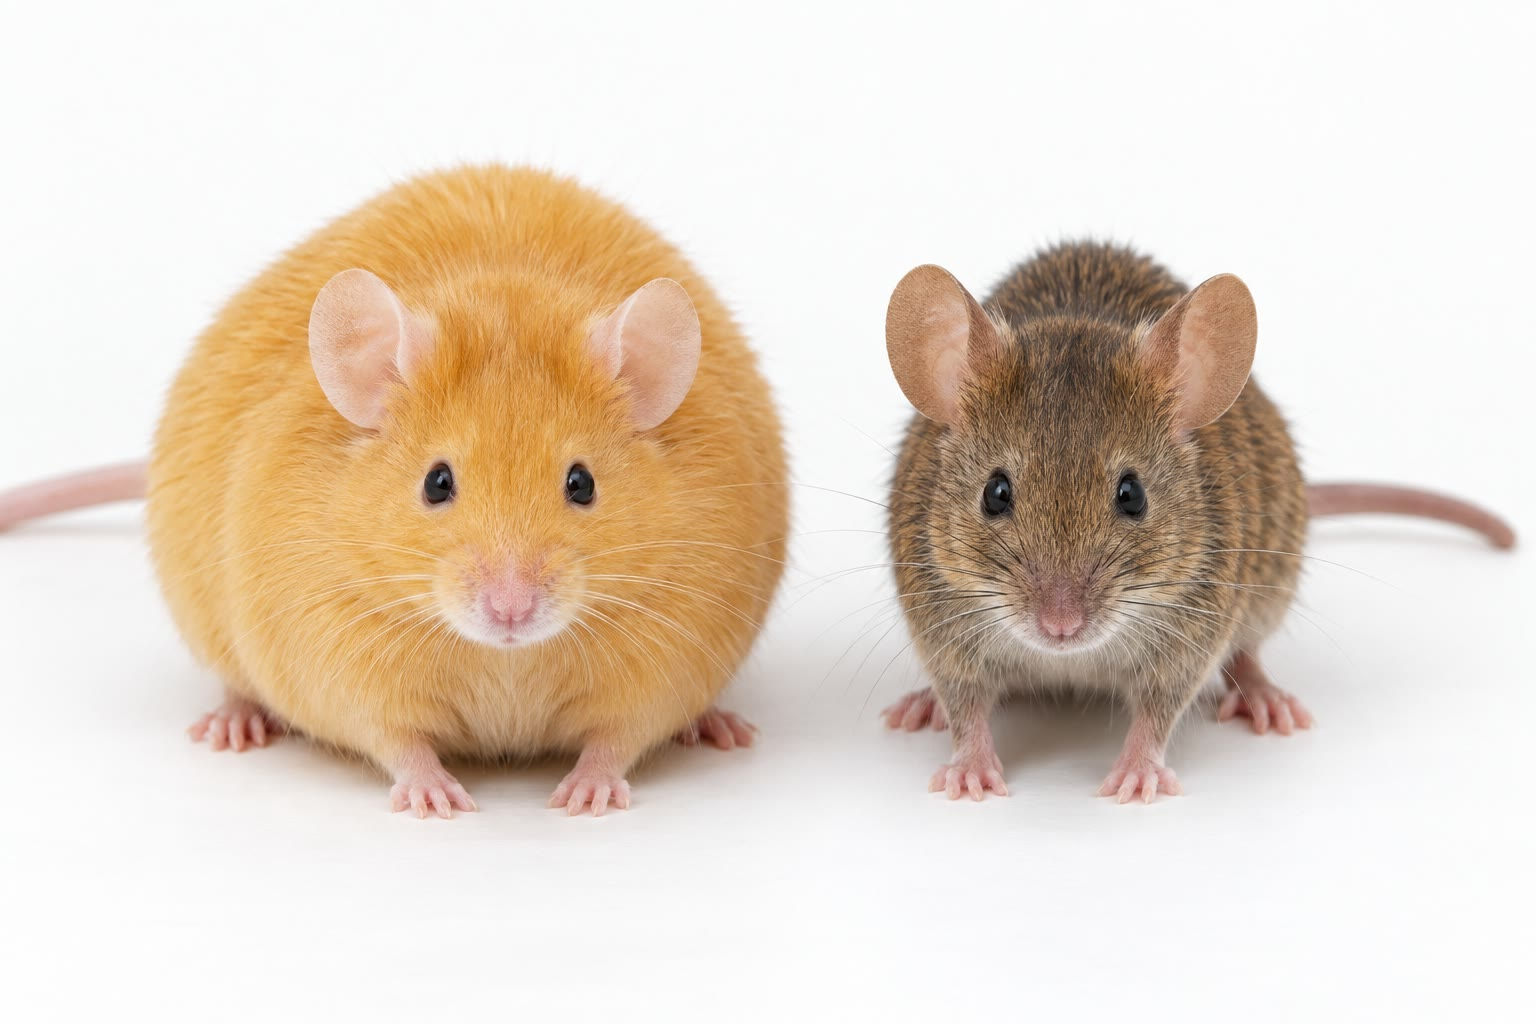
\includegraphics[width=0.62\linewidth]{images/book5/ai/b5-01-agouti-mice.jpg}

{\small 两只基因型相同的 $A^{vy}$ 同窝小鼠：一只黄色肥胖的
小鼠，其 \emph{agouti} 上游的转座子未甲基化，
另一只为棕色“假刺鼠色”小鼠，其转座子已甲基化。}
\end{omfigure}

\begin{proposition}[可遗传表观遗传状态的实例]\label{prop:b3:chromatin-epigenetics:examples}
\index{位置效应花斑}\index{春化作用}\index{副突变}
三个研究充分的体系说明了上述机制。
\emph{\omterm{prop:b3:chromatin-epigenetics:examples}{位置效应花斑}}见于 \emph{Drosophila}：一个基因因染色体重排
被移到\omterm{def:b3:chromatin-epigenetics:nucleosome}{异染色质}旁，在部分细胞中被沉默，而在其他细胞中则不然，
形成斑驳的眼色；每个斑块都是一个克隆，沉默由\omterm{def:b3:chromatin-epigenetics:nucleosome}{异染色质}
经 \omterm{prop:b3:chromatin-epigenetics:readers}{HP1} 环向外扩散；其突变能抑制花斑的基因
（\emph{Su(var)} 基因）为
\omterm{prop:b3:chromatin-epigenetics:readers}{HP1} 与 H3K9 甲基转移酶。
\emph{\omterm{prop:b3:chromatin-epigenetics:examples}{春化作用}}见于 \emph{Arabidopsis}：数周的冬季低温
通过 Polycomb 沉积的 H3K27me3 沉默开花抑制因子 \emph{FLC}，
这种沉默可持续数月的春季生长，
历经数千次细胞分裂，并在每一代被重置，
使每株植物都必须经历自己的冬季。\emph{\omterm{prop:b3:chromatin-epigenetics:examples}{副突变}}见于
玉米：\emph{b1} 色素基因的一个等位基因，与杂合子中
某一特定的其他等位基因相遇时，会将其转变为自身的沉默状态，
而被转变的等位基因又将这一状态传递给后代数代，
这一过程通过小 RNA 指导的甲基化完成，
该机制在\cref{ch:b3:rna-regulation}中讨论。在上述每种情形中，
遗传均为有丝分裂式且稳健；跨代传递则
或被主动重置（植物），或为渗漏、不完全的（小鼠）。
\end{proposition}

\begin{remark}[跨代说法的局限]\label{rem:b3:chromatin-epigenetics:limits}
认为祖父母的饥荒或应激“通过表观遗传”传给人类孙辈的说法
十分常见，但大多尚未得到证实。
体细胞标记与孙辈之间隔着两轮抹除，
印记基因与少数转座子是哺乳动物中仅有的、
经证实能在抹除中留存的成分；在人类队列中，
共享环境、子宫环境与遗传差异的效应，
很难与种系所携带的标记区分开来。
已证实的情形——$A^{vy}$、部分与转座子相关的
\omterm{def:b3:chromatin-epigenetics:epigenetics}{表观等位基因}，以及线虫和植物中由 RNA 介导的状态——确实存在，
分子机制清楚，适用范围狭窄。本章定理说明了原因：
若无一种将 $\mu$ 推向 $1$ 的反馈，标记会在
几十次分裂内自行遗忘，而种系还会额外施加一次主动重置。
\end{remark}

\section{练习}

\begin{exercise}[$\star$]\label{exo:b3:chromatin-epigenetics:1}
写出\omterm{def:b3:chromatin-epigenetics:nucleosome}{核小体}核心颗粒的组成、它所结合的 DNA 长度，
以及典型的连接子长度。为什么用核酸酶消化\omterm{def:b3:chromatin-epigenetics:nucleosome}{染色质}得到的是梯状片段，
而不是弥散的条带？
\end{exercise}

\begin{exercise}[$\star$]\label{exo:b3:chromatin-epigenetics:2}
某种蛙的基因组每个单倍体组含 $3.0\times 10^{9}$ 个碱基对。
求二倍体细胞核中含有多少个\omterm{def:b3:chromatin-epigenetics:nucleosome}{核小体}（取重复单元为
\qty{190}{bp}），以及其 DNA 的长度。
\end{exercise}

\begin{exercise}[$\star$]\label{exo:b3:chromatin-epigenetics:3}
解读 H3K27me3、H4K16ac 和 H3S10ph。对每一种标记，说明它与
活跃\omterm{def:b3:chromatin-epigenetics:nucleosome}{染色质}还是沉默\omterm{def:b3:chromatin-epigenetics:nucleosome}{染色质}相关，并为第一种标记
指出一个\omterm{def:b3:chromatin-epigenetics:histone-code}{阅读器}。
\end{exercise}

\begin{exercise}[$\star$]\label{exo:b3:chromatin-epigenetics:4}
解释为什么三色猫几乎总是雌性，
以及一只雄性三色猫必须具有怎样的核型。
\end{exercise}

\begin{exercise}[$\star\star$]\label{exo:b3:chromatin-epigenetics:5}
利用 \qty{10}{nm} 纤维的数据计算其堆积比，
数据取自\cref{def:b3:chromatin-epigenetics:nucleosome}（重复单元 \qty{200}{bp}，
珠粒直径 \qty{11}{nm}），再计算将一条平均大小的人类染色体中长 \qty{4}{cm} 的 DNA 装入
长 \qty{4}{\micro m} 的有丝分裂染色单体所需的堆积比，
纤维还需再折叠多少倍？
\end{exercise}

\begin{exercise}[$\star\star$]\label{exo:b3:chromatin-epigenetics:6}
在\cref{thm:b3:chromatin-epigenetics:maintenance}的模型中，
取 $\mu = 0.98$，$\delta = 0.01$，求 $p^{*}$，以及
从一开始即甲基化的位点丢失其
超出 $p^{*}$ 部分的一半时所经历的分裂次数。对 $\mu = 0.999$，$\delta = 0.001$，重复上述计算。
\end{exercise}

\begin{exercise}[$\star\star$]\label{exo:b3:chromatin-epigenetics:7}
对肝细胞进行 ChIP-seq 实验，结果显示 H3K4me3 峰和
H3K27ac 峰位于基因 $A$ 的启动子处，基因 $B$ 上有一个宽的 H3K27me3 区域，
基因 $C$ 上有 H3K9me3。预测三者各自的转录状态，
并说明 $B$ 与 $C$ 中哪一个更可能在另一种细胞类型中被激活，
并解释原因。
\end{exercise}

\begin{exercise}[$\star\star$]\label{exo:b3:chromatin-epigenetics:8}
一名女性在一条 15 号染色体上携带 \emph{UBE3A} 区域的缺失，但身体健康。
她的父亲携带相同的缺失，同样身体健康。
若有的话，她的每个孩子各面临哪种综合征的风险，
概率分别为多少？如果这一缺失来自她的母亲，
情况又会如何？
\end{exercise}

\begin{exercise}[$\star\star$]\label{exo:b3:chromatin-epigenetics:9}
预测在雌性小鼠胚胎中，删除
\emph{\omterm{def:b3:chromatin-epigenetics:x-inactivation}{Xist}} 基因分别来自一条或两条 X 染色体时的后果，并预测将
\emph{\omterm{def:b3:chromatin-epigenetics:x-inactivation}{Xist}} 转基因插入一条常染色体后，该常染色体会发生什么变化。
\end{exercise}

\begin{exercise}[$\star\star\star$]\label{exo:b3:chromatin-epigenetics:10}
结合\cref{ex:b3:chromatin-epigenetics:cpg-deficit}，解释为什么 \omterm{def:b3:chromatin-epigenetics:methylation}{CpG} 岛保留了其中的 \omterm{def:b3:chromatin-epigenetics:methylation}{CpG}，
而基因组其余部分却丢失了其中五分之四；
并说明这对种系中 \omterm{def:b3:chromatin-epigenetics:methylation}{CpG} 岛在进化时间尺度上的甲基化状态意味着什么。
为什么这一论证不适用于
仅在肝脏中被甲基化的基因？
\end{exercise}

\begin{exercise}[$\star\star\star$]\label{exo:b3:chromatin-epigenetics:11}
利用\omterm{def:b3:chromatin-epigenetics:histone-code}{书写器}–\omterm{def:b3:chromatin-epigenetics:histone-code}{阅读器}循环，说明 H3K9me3 结构域
如何在复制过程中保持稳定（见\cref{prop:b3:chromatin-epigenetics:readers}），
尽管每次分裂都会使带标记的\omterm{def:b3:chromatin-epigenetics:nucleosome}{组蛋白}被未带标记的新\omterm{def:b3:chromatin-epigenetics:nucleosome}{组蛋白}
稀释为原来的一半。是什么决定该结构域
停止扩展的位置？请提出一个实验来检验你的解释。
\end{exercise}

\begin{exercise}[$\star\star\star$]\label{exo:b3:chromatin-epigenetics:12}
一项研究报告称，经历过饥荒的人的孙辈
在一个生长基因上的甲基化发生了改变，且体重更高。
在断定甲基化标记已通过种系传递之前，需排除的
其他解释有哪些；
并说明应以怎样的小鼠实验来解决这一问题。
\end{exercise}

\section{问题：沉默基因的记忆}

\begin{problem}[{周末问题——装入细胞核的人类基因组，
随分裂追踪的甲基化标记，将三色猫读作克隆图谱，
以及统计印记区域的疾病，
最后归结到无反馈时标记能存活的分裂次数，
以及选择其 X 染色体的细胞群体大小}]
\label{pb:b3:chromatin-epigenetics:1}
数据：人类二倍体细胞核含有 $6.4\times 10^{9}$ 个碱基对，每对长 \qty{0.34}{nm}、质量为 \qty{650}{Da}；
\omterm{def:b3:chromatin-epigenetics:nucleosome}{核小体}重复单元为 \qty{200}{bp}，\omterm{def:b3:chromatin-epigenetics:nucleosome}{组蛋白}八聚体质量为 \qty{108}{kDa}，
核心颗粒为直径 \qty{11}{nm}、厚 \qty{5.5}{nm} 的圆盘。
细胞核为直径 \qty{10}{\micro m} 的球体。
该基因组的 G$+$C 含量为 \qty{42}{\%}。
普通 \omterm{def:b3:chromatin-epigenetics:methylation}{CpG} 位点的甲基化：$\mu = 0.99$，
每次分裂 $\delta = 0.02$。

\medskip
\noindent\textbf{第一部分——堆积。}
\begin{enumerate}
  \item 计算细胞核中 DNA 的总长度，
        以及\omterm{def:b3:chromatin-epigenetics:nucleosome}{核小体}的数目。
  \item 计算\omterm{def:b3:chromatin-epigenetics:nucleosome}{组蛋白}（仅八聚体）和 DNA 的总质量，
        单位为皮克（$\qty{1}{Da} = \qty{1.66e-24}{g}$）。
  \item 计算细胞核的体积，以及将核心颗粒视为圆柱体后的
        总体积，
        它们占细胞核的比例是多少？
  \item 若将\omterm{def:b3:chromatin-epigenetics:nucleosome}{核小体}首尾相接，排成直径为 \qty{10}{nm} 的
        纤维，则该纤维有多长，
        相对于裸露 DNA 的堆积比是多少？
  \item 纤维被折叠成由黏连蛋白锚定的 \qty{200}{kb} 环，
        共有多少个环，每个环含多少个\omterm{def:b3:chromatin-epigenetics:nucleosome}{核小体}？
  \item 在独立性假设下，二倍体基因组中会含有多少个 \omterm{def:b3:chromatin-epigenetics:methylation}{CpG} 二核苷酸？
        观测到的数目为
        $5.6\times 10^{7}$。已丢失的比例是多少，
        由哪种突变机制造成？
\end{enumerate}

\medskip
\noindent\textbf{第二部分——分裂中传递的标记。}
\begin{enumerate}[resume]
  \item 写出 $p_{n}$ 的递推关系，并求 $p^{*}$。
  \item 启动子 \omterm{def:b3:chromatin-epigenetics:methylation}{CpG} 在 $n = 0$ 时完全甲基化，求 $p_{n}$
        在分裂 $10$、$50$ 和 $200$ 次后的值。
  \item 经过多少次分裂后，过量 $p_{n} - p^{*}$ 减半？
        组织干细胞约每周分裂一次，这相当于
        多少年？
  \item 某药物完全抑制 \omterm{def:b3:chromatin-epigenetics:methylation}{DNMT1}（$\mu = 0$），也完全抑制 DNMT3
        （$\delta = 0$）。证明：群体中甲基化链的比例
        在每次分裂时减半，并求将甲基化水平由 \qty{80}{\%}
        降至 \qty{5}{\%} 以下所需的分裂次数。
  \item 在沉默岛中，甲基化 \omterm{def:b3:chromatin-epigenetics:methylation}{CpG} \omterm{def:b3:chromatin-epigenetics:histone-code}{阅读器}招募 H3K9
        甲基化，后者再招募 DNMT3，使岛内
        $\mu = 0.9995$，$\delta = 0.0005$，重新计算
        过量部分的半衰期，分别以分裂次数和
        每周一次分裂对应的年数表示。
  \item 用一句话说明，为何终身沉默的基因需要的是第 11 题的结果，而非
        第 9 题的结果，并说明产生它的是哪种
        分子层面的机制。
\end{enumerate}

\medskip
\noindent\textbf{第三部分——三花猫的斑块图。}
\begin{enumerate}[resume]
  \item 某只雌猫在 X 连锁的橙色基因上为杂合子。说明
        其毛皮为何有橙色和黑色斑块，以及每一块斑块
        代表什么。
  \item X 染色体失活发生于将形成皮肤的细胞
        数为 $N$ 时，每个细胞随机选择一条 X 染色体。
        求所有 $N$ 个细胞选中同一条 X 染色体的概率，
        即得到单色猫的概率。
  \item 迄今未见此类单色杂合雌猫的记录，
        全球猫的数量或约十亿只；取概率为
        $10^{-9}$，估算 $N$。
  \item 该猫的皮肤表面积约为 \qty{0.3}{m^2}，其斑块
        平均面积为 \qty{15}{cm^2}。估算斑块数目，并
        说明它为何大于 $N$。
  \item 一只 XXY 雄猫同样是三花猫。他的细胞中
        有多少个\omterm{def:b3:chromatin-epigenetics:x-inactivation}{巴氏小体}？XXX 雌性和 XY 雄性各有多少个？
  \item 逃避失活的基因在雌性中有两个活性拷贝，
        在雄性中有一个。试给出此类逃逸可被容忍的一个
        理由，并给出一种其影响不可忽视的情形。
\end{enumerate}

\medskip
\noindent\textbf{第四部分——第 15 号染色体。}
\begin{enumerate}[resume]
  \item 普拉德–威利综合征约每
        \num{15000} 例出生中有一例；\qty{70}{\%} 的病例为
        父源 15q11--q13 的从头缺失，\qty{25}{\%} 为母源
        \omterm{def:b3:chromatin-epigenetics:imprinting}{单亲二体}。计算每种病因的出生频率。
  \item 天使综合征的频率与之大致相同；\qty{70}{\%}
        为母源缺失，\qty{5}{\%} 为父源\omterm{def:b3:chromatin-epigenetics:imprinting}{单亲二体}，
        \qty{10}{\%} 为 \emph{UBE3A} 的点突变。为何点突变
        是天使综合征的病因，却几乎从不导致普拉德–威利综合征？
  \item 某父亲携带平衡易位，使
        \qty{20}{\%} 的精子携带 15q11--q13 缺失。
        其子女中患普拉德–威利综合征和天使综合征的比例各为多少？
  \item 当三体受精卵丢失一条染色体时，便产生\omterm{def:b3:chromatin-epigenetics:imprinting}{单亲二体}。
        若 15 号三体受精卵随机丢失其三条
        染色体中的一条，且三体来源于母亲（两条母源拷贝），
        则幸存者为母源\omterm{def:b3:chromatin-epigenetics:imprinting}{单亲二体}的概率是多少？
        属于哪种综合征？
  \item 普拉德–威利综合征相关基因为父源表达，天使综合征
        相关基因为母源表达。运用亲缘关系学说，指出
        两种综合征的症状中，哪些（出生时喂养困难与
        对比食欲旺盛）符合该学说，哪些
        较难与之吻合。
  \item 有人提出一种治疗天使综合征的方法：重新激活
        沉默的父源 \emph{UBE3A}。其沉默由父源表达的
        反义 RNA 所致。试提出分子靶点，并说明
        该疗法为何不会干扰其他印记基因。
  \item 总结：无反馈时标记的半衰期（第 9 题）和
        有反馈时的半衰期（第 11 题），以分裂次数计；以及
        三花猫毛色的奠基者种群大小 $N$（第 15 题）。
\end{enumerate}
\end{problem}
